\documentclass{article}
\usepackage[utf8]{inputenc}
\PassOptionsToPackage{hyphens}{url}
\usepackage{hyperref}
\usepackage{algorithmic}
\usepackage{graphicx, animate}
\usepackage{listings}

\graphicspath{ {./imagini/}}

\title{Tema 2 - Computer Networks LNCS Documentantion}
\author{Niță Dennis-Alexandru}
\date{11 Decembrie 2023}

\usepackage{listings}
\usepackage{color}

\definecolor{dkgreen}{rgb}{0,0.6,0}
\definecolor{gray}{rgb}{0.5,0.5,0.5}
\definecolor{mauve}{rgb}{0.58,0,0.82}

\lstset{frame=tb,
  language=C++,
  aboveskip=3mm,
  belowskip=3mm,
  showstringspaces=false,
  columns=flexible,
  basicstyle={\small\ttfamily},
  numbers=none,
  numberstyle=\tiny\color{gray},
  keywordstyle=\color{blue},
  commentstyle=\color{dkgreen},
  stringstyle=\color{mauve},
  breaklines=true,
  breakatwhitespace=true,
  tabsize=3
}

\begin{document}

\maketitle

{\Large \bf 1 Introducere} 
\\

Proiectul pe care mi l-am ales este despre o aplicație client/server care permite editarea simultană a fișierelor text.
Serverul trebuie să permită creearea simultană a mai multor "camere" în care doi clienți pot prelucra fișiere text, simultan.
\\

{\Large \bf 2 Tehnologii Aplicate} 
\\


Pentru acest proiect am folosit limbajul {\bf C++} standardul 2017 compilat cu {\bf g++ 13.1.0} pe distro-ul {\bf Ubuntu 23.0}. Motivația alegerii acestui limbaj a fost
accesul la programarea orientată pe obiecte, drept și librăriile aferente lui. Ca și protocol de comunicație, am ales protocolul {\bf TCP} deoarece
pentru acest gen de aplicație este nevoie de un stream constant de informații, actualizarea {\bf notepad-ului} fiind făcută în timp real.
Thread-ul main al procesului executat este serverul propriu-zis, acesta ascultând după conecțiuni noi de la clienți. În urma conectării unui client,
se creează un thread noi specific acelui client care va asculta informațiile de la client, le va prelucra și va trimite înapoi la client un răspuns.

Pentru interfața grafică a clientului (serverul nu are interfață grafică) am folosit {\bf SFML 2.6.1} deoarece este o librărie puternică, care satură nevoile grafice ale acestui proiect.
\\

\newpage

{\Large \bf 3 Structura aplicației} 
\\

{\Large Diagrama TCP}


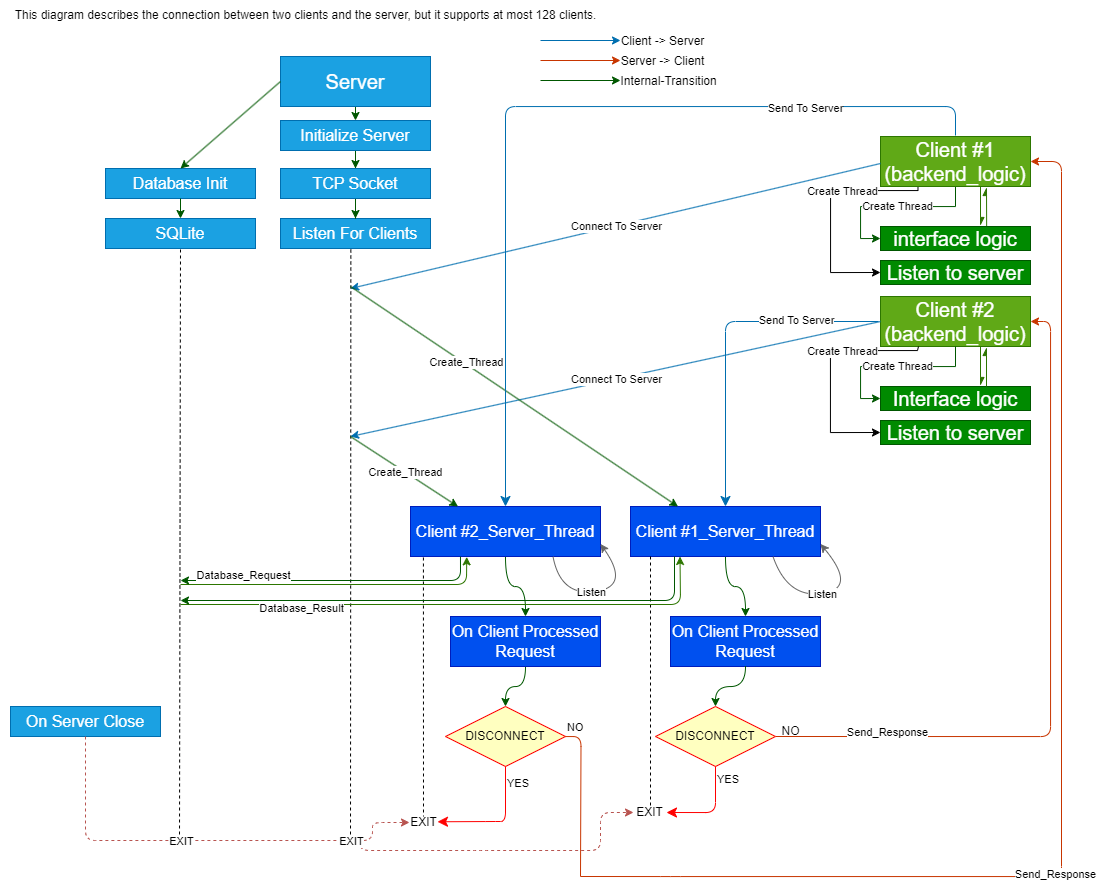
\includegraphics[scale=0.403]{tcp.png}


\newpage
{\Large Diagrama UML}


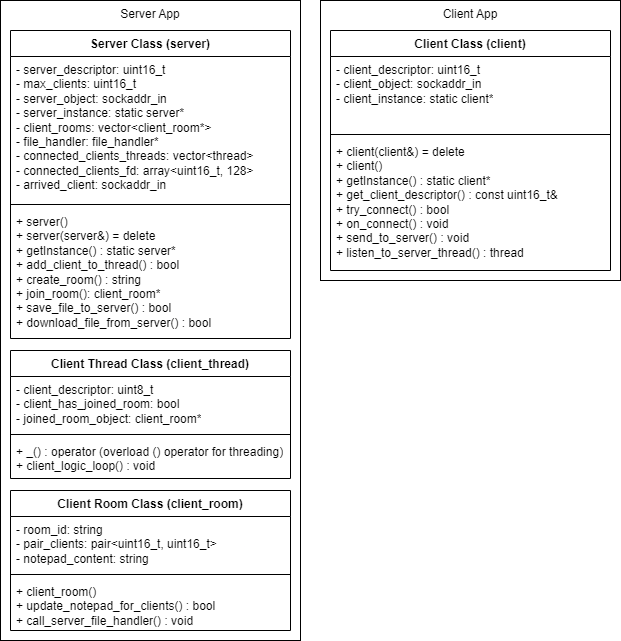
\includegraphics[scale=0.529]{uml.png}

\newpage
{\Large \bf 4 Aspecte de implementare} 

Pentru acest proiect am implementat partea de server/client cu librăriile {\bf UNIX} (ex: sys/socket, netinet/ip.h) și drept design-pattern;
serverul și clientul sunt singleton-uri pentru că orice instanță a aplicației client sau a aplicație server au, implicit, un singur client sau un singur server.
\\

{\large server.cpp}
\begin{lstlisting}
    class server
    {
    private:
        // members described in UML diagram
    public:
        ...
        server(#parameters)
        {
            ...
        }
    
        static server* instance(#parameters)
        {
            if(server_instance == nullptr)
            {
                server_instance = new server(_sock_type, _sock_stream, _protocol, _htonl, _port, _max_clients);
            }
            return server_instance;
        }
    
        static server* instance()
        {
            if(server_instance != nullptr)
            {
                return server_instance;
            }
            handle_error("An unexceptional error occured: No server.\n");
        }

        //function defined in UML diagram
    }
\end{lstlisting}

\newpage
{\large client.cpp}
\begin{lstlisting}
    class client
    {
    private:
        // members described in UML diagram
    public:
        ...
        client(#parameters)
        {
            ...
        }
    
        static client* client(#parameters)
        {
            if(client_instance == nullptr)
            {
                client_instance = new client(_sock_type, _sock_stream, _protocol, _ip_adress, _port);
            }
            return client_instance;
        }
    
        static client *instance()
        {
            if(client_instance != nullptr) 
                return client_instance;
        }

        //function defined in UML diagram
    }
    \end{lstlisting}

\newpage
{\Large \bf 5 Concluzii}
\\

Concluzia este.
12345
\\

{\Large \bf 6 Refererințe bibliografice}
\\

Mama sita porfavor


\end{document}